\section{Modeling NASA-TLX Weighted Scores and Subscales}
\label{apdx:model_tlx}
This section first describes the hierarchical Bayesian ordinal regression model used for the NASA-TLX weighted scores and subscales. We then present the results for each subscale.

\subsection{Modeling Approach}

\subsubsection{Dependent variables}
\paragraph{NASA-TLX weighted scores} are transformed from a continuous $0$--$100$ scale to cognitive levels: low, medium, somewhat high, high, and very high, as described by~\citet{hart1988development}. This transformation helps the model adapt to sparse data. In our study, there were no participants who expressed "low" or "very high"; thus, we modeled the predictive variables as "medium," "somewhat high," and "high."

\paragraph{NASA-TLX subscale ratings} are transformed into ordinal groups using minimum frequency binning~\cite{frank2001simple}. Minimum frequency binning involves grouping adjacent response categories until each bin meets a predefined minimum number of observations. Since the subscale uses a 21-point Likert scale and we have 40 participants, the data are very sparse. Minimum frequency binning mitigates this by ensuring similar numbers of participants in each bin. We applied weighted bins across all participants within the same subscale, ensuring that each bin contained at least 10 participants.

\paragraph{Likelihood.} With these ordinal outcome variables, we designed $y_i$ as the observed ordinal category for participant $i$. Then:

\begin{equation}
    y_i \sim \text{OrderedLogistic}(\eta_i, \boldsymbol{\tau}),
    \label{eq:cog_main}
\end{equation}

where $\eta_i$ is the latent predictor, and $\boldsymbol{\tau}$ denotes the cutpoints demarcating the boundaries between the ordinal categories as in~\Cref{eq:cog_orderedTransfrom}. The cutpoints $\boldsymbol{\tau}$ ensure that $\tau_1 < \tau_2 < \cdots < \tau_{K-1}$ by construction.

\begin{equation}
    \boldsymbol{\tau} \sim \text{OrderedTransform}(\mathcal{N}(0, 1)^{K-1}),
    \label{eq:cog_orderedTransfrom}
\end{equation}

\subsubsection{Independent Variables and latent predictor}
For this model, we used three independent variables: length ($\gamma_i$, an ordinal variable), interface type ($\beta_I$, an categorical variable), and the interaction between the two ($\phi_{i,j}$) to construct the latent predictor $\eta_i$. Specifically, the latent predictor $\eta_i$ is constructed as:

\begin{equation}
    \eta_i = \alpha + \gamma_i + \beta_I[I_i] + \phi_{i,j},
    \label{eq:cog_regression}
\end{equation}

where: $\alpha$ is a global intercept drawn from $\mathcal{N}(0,1)$, $\gamma_i$ captures the (ordinal) effect of length, $\beta_I[I_i]$ is the effect for interface $I_i$, and $\phi_{i,j}$ is the interaction between length $i$ and interface $j$. 

Since length has two levels (short and long), we define the following equation to account for ordinality:
\begin{equation}
    \gamma_i = \mu_L + \beta_L \cdot L_i
    \label{eq:cog_ordinal}
\end{equation}

where $L_i \in \{0,1\}$, making $\gamma_i = \mu_L$ for the short condition and $\gamma_i = \mu_L + \beta_L$ for the long condition. We assign standard normal priors to these parameters: $\mu_L \sim \mathcal{N}(0,1)$ and $\beta_L \sim \mathcal{N}(0,1)$. 

\paragraph{Interface Effects.}
We model the interface effects using a non-centered parameterization to improve numerical stability and encourage partial pooling across the two interface levels. Specifically, we let $\mu_{\beta_I} \sim \mathcal{N}(0,1)$ and $\sigma_{\beta_I} \sim \mathrm{Exponential}(1)$ represent the shared mean and scale of the interface effects. We then sample a raw effect vector $\beta_{I_{\text{raw}}} \sim \mathcal{N}(0,1)^2.$ Combining these, we define:
\begin{equation}
    \beta_I = \mu_{\beta_I} + \sigma_{\beta_I} \cdot \beta_{I_{\text{raw}}}
    \label{eq:interface_reparam}
\end{equation}
where $\beta_I \in \mathbb{R}^2$ contains the effect for each of the two interface levels, 
and $\beta_I[I_i]$ indexes the effect for participant $i$'s interface. 

\paragraph{Interaction Effects} To capture potential interaction effects between length and interface types, we assign one interaction parameter, $\phi_{i,j}$, to each combination of length $i$ and interface $j$. Rather than sampling these $\phi_{i,j}$ directly, we employ a non-centered parameterization:
\[
  \boldsymbol{\phi} = L_{\Omega} \,\bigl(\sigma_{\phi} \odot z_{\phi}\bigr),
\]
where \(\boldsymbol{\phi}\) is a $2 \times 2$ matrix of interaction parameters (since we have 2 levels of length and 2 levels of interface), $z_{\phi} \sim \mathcal{N}(0,1)^{2\times2}$, $\sigma_{\phi} \sim \text{Exponential}(1)^{2\times2}$, and $L_{\Omega}$ is the Cholesky factor of a correlation matrix drawn from an $\text{LKJ}(2)$ prior. We then define
\[
    \phi_{i,j} 
    = 
    \bigl[\boldsymbol{\phi}\bigr]_{i,j},
\]
making $\phi_{i,j}$ a \emph{single scalar} drawn from the correlated matrix $\boldsymbol{\phi}$.

\subsubsection{Posterior predictive plots}
We conducted the Bayesian analysis using NumPyro, a widely used framework for Bayesian inference. We used Markov Chain Monte Carlo (MCMC) sampling, a method commonly applied in Bayesian inference. The model converged successfully, as evidenced by an $\hat{R}$ value of 1 for each subscale and the overall weighted TLX scores, indicating that multiple sampling chains converged. We plotted the posterior predictive distribution of the model to compare the observed data with the model's predictions. Figure~\ref{fig:observed_vs_predicted_all_subscale} shows the posterior predictions vs. observed data for the six subscales.

\begin{figure*}[h!]
    \centering
    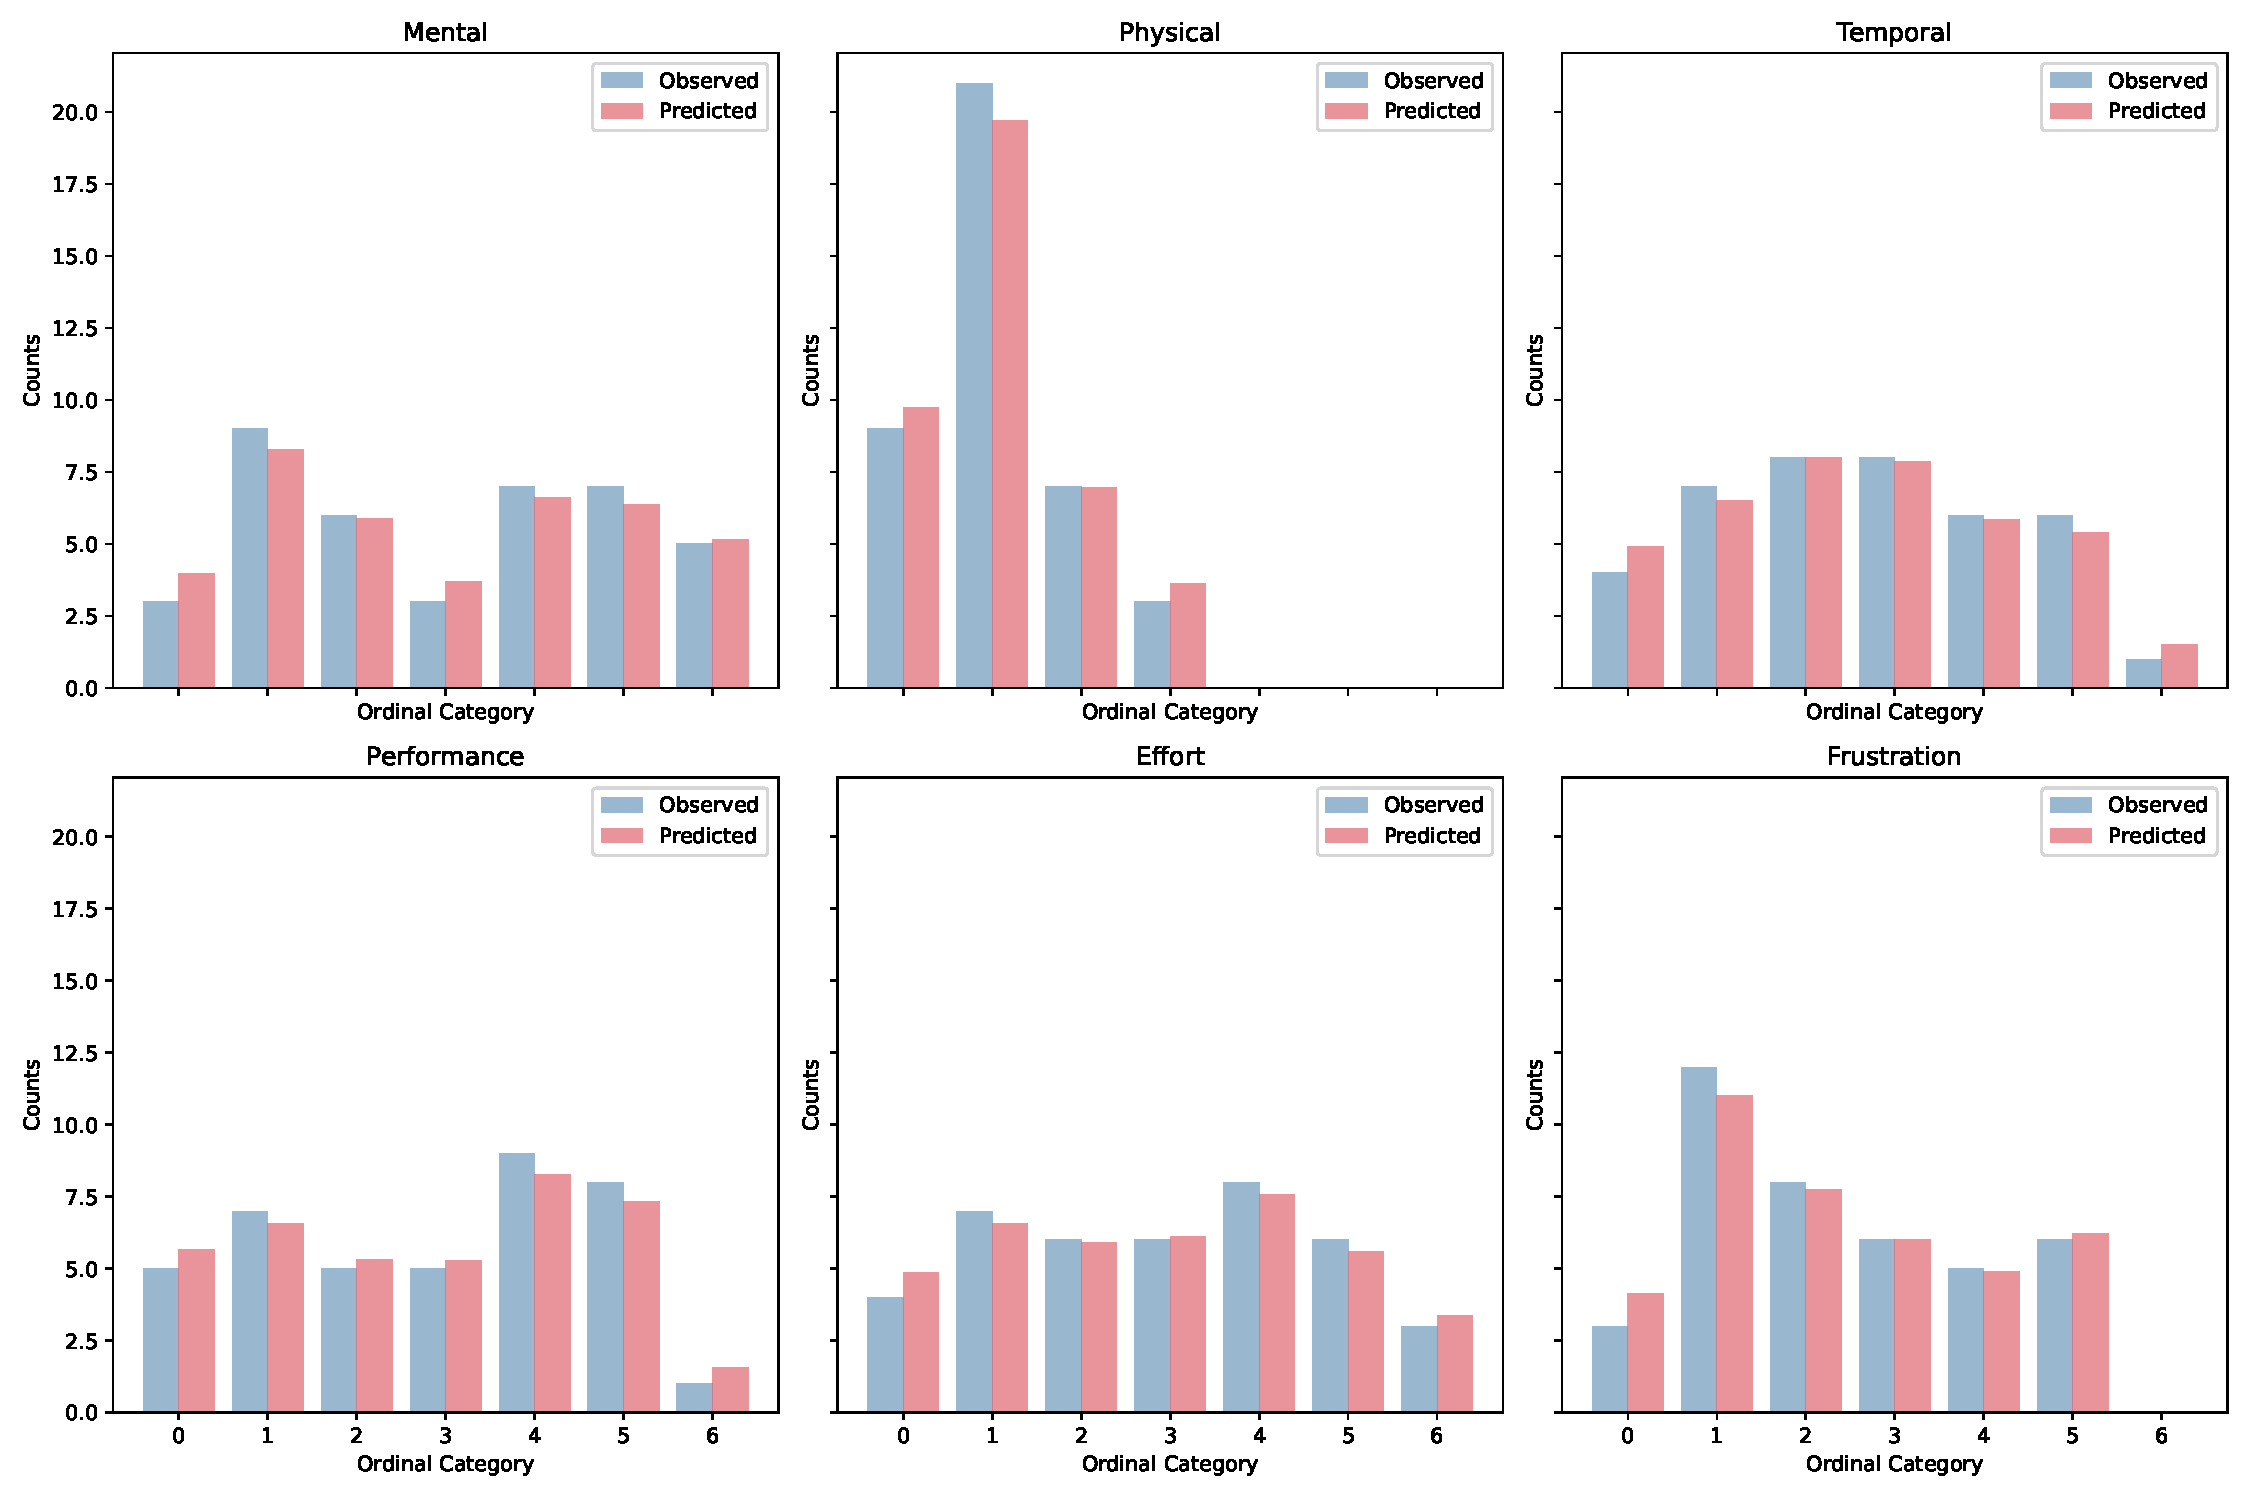
\includegraphics[width=\textwidth]{content/image/cog/observed_vs_predicted_all_subscale.pdf}
    \caption{Posterior Predictions vs. observed data for NASA-TLX subscales. The plot shows the observed number of participants in each bin compared to the posterior predictions from the model. \textbf{Takeaway of the plot}: We believe that the model is reasonable at capturing the distribution of the subscales given the sparsity of the data.}
    \Description{ A collection of bar charts comparing observed versus predicted counts across six subscales: Mental, Physical, Temporal, Performance, Effort, and Frustration. Each chart compares counts (y-axis) across ordinal categories (x-axis), highlighting discrepancies between observed and predicted values for each subscale. Bars are color-coded to distinguish observed and predicted values.}
    \label{fig:observed_vs_predicted_all_subscale}
\end{figure*}

\subsection{Model Results}
\begin{figure*}[h!]
    \centering
    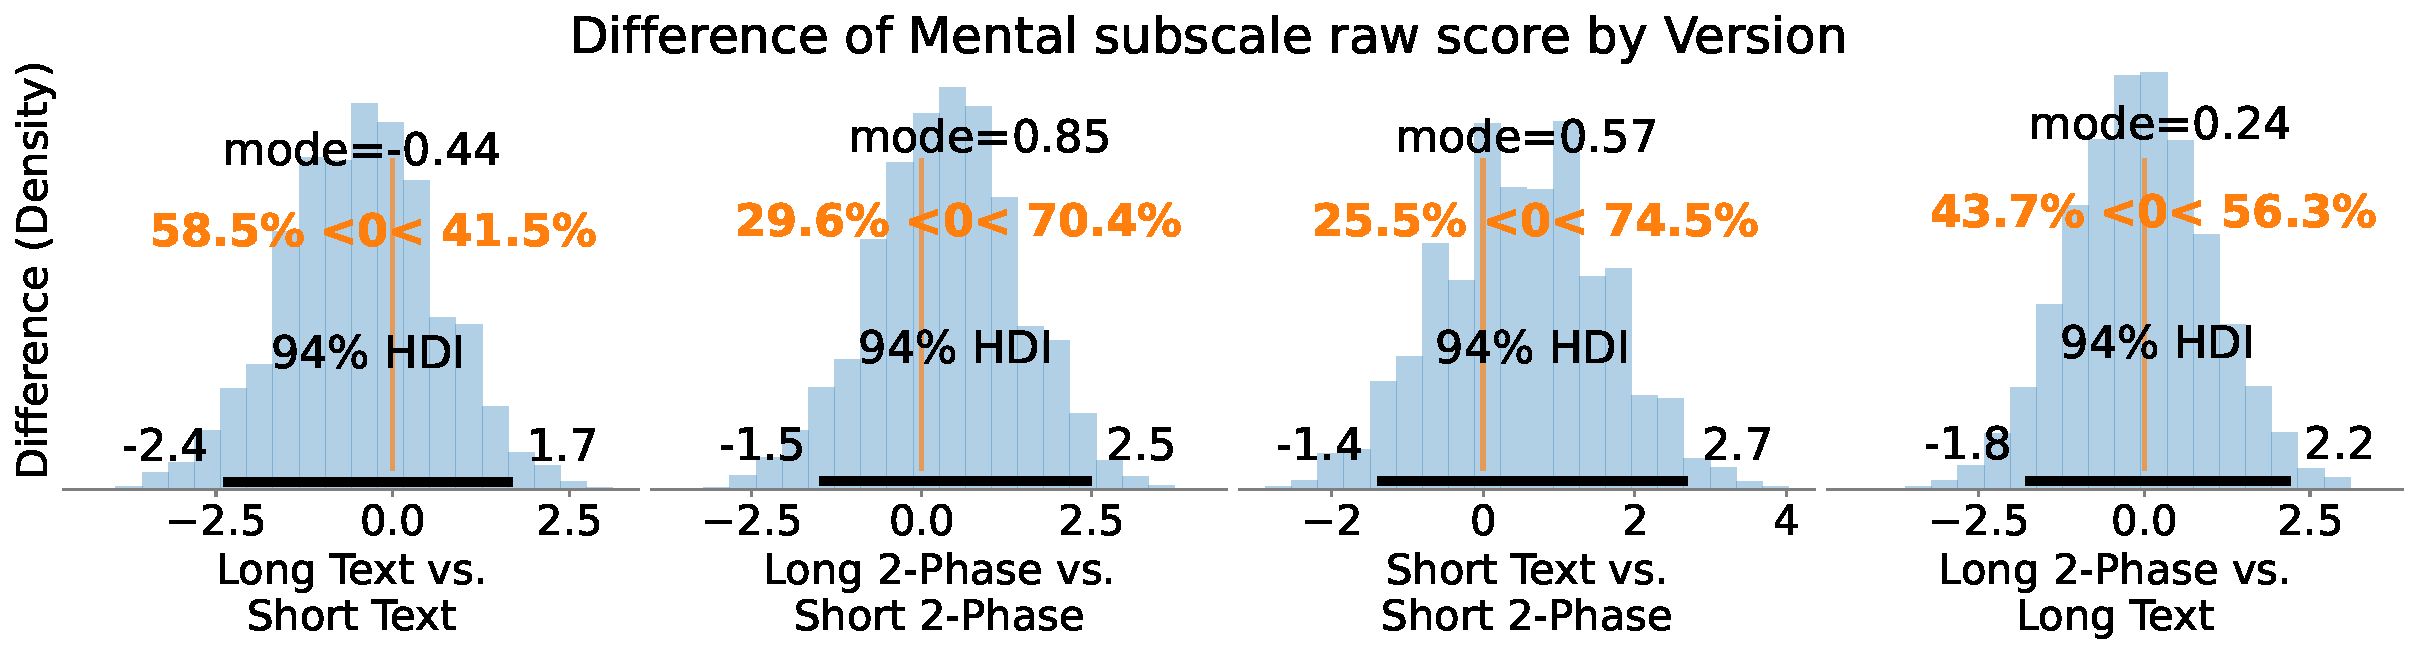
\includegraphics[width=0.75\textwidth]{content/image/cog/Mental_cog_diff_single_row.pdf}
    \caption{Differences in the mental subscale scores by version.~\textbf{Main Takeaway:} Participants in the long two-phase condition show trends to increase mental demand compared to the short two-phase. Within the short text condition, participants in the short two-phase condition show a trend to reduce mental demand.}
    \Description{A grouped panel of four histograms titled "Difference of Mental subscale raw score by Version," displaying posterior distributions of differences between various experimental conditions. Each plot shows a histogram of density (y-axis) versus difference (x-axis), with key summary statistics. Each histogram includes credible intervals, density curves, and a vertical line at zero for reference. Summary values are highlighted in orange and positioned at the top of each plot.}
    \label{fig:bayesian_mental_subscale}
\end{figure*}

\begin{figure*}[h!]
    \centering
    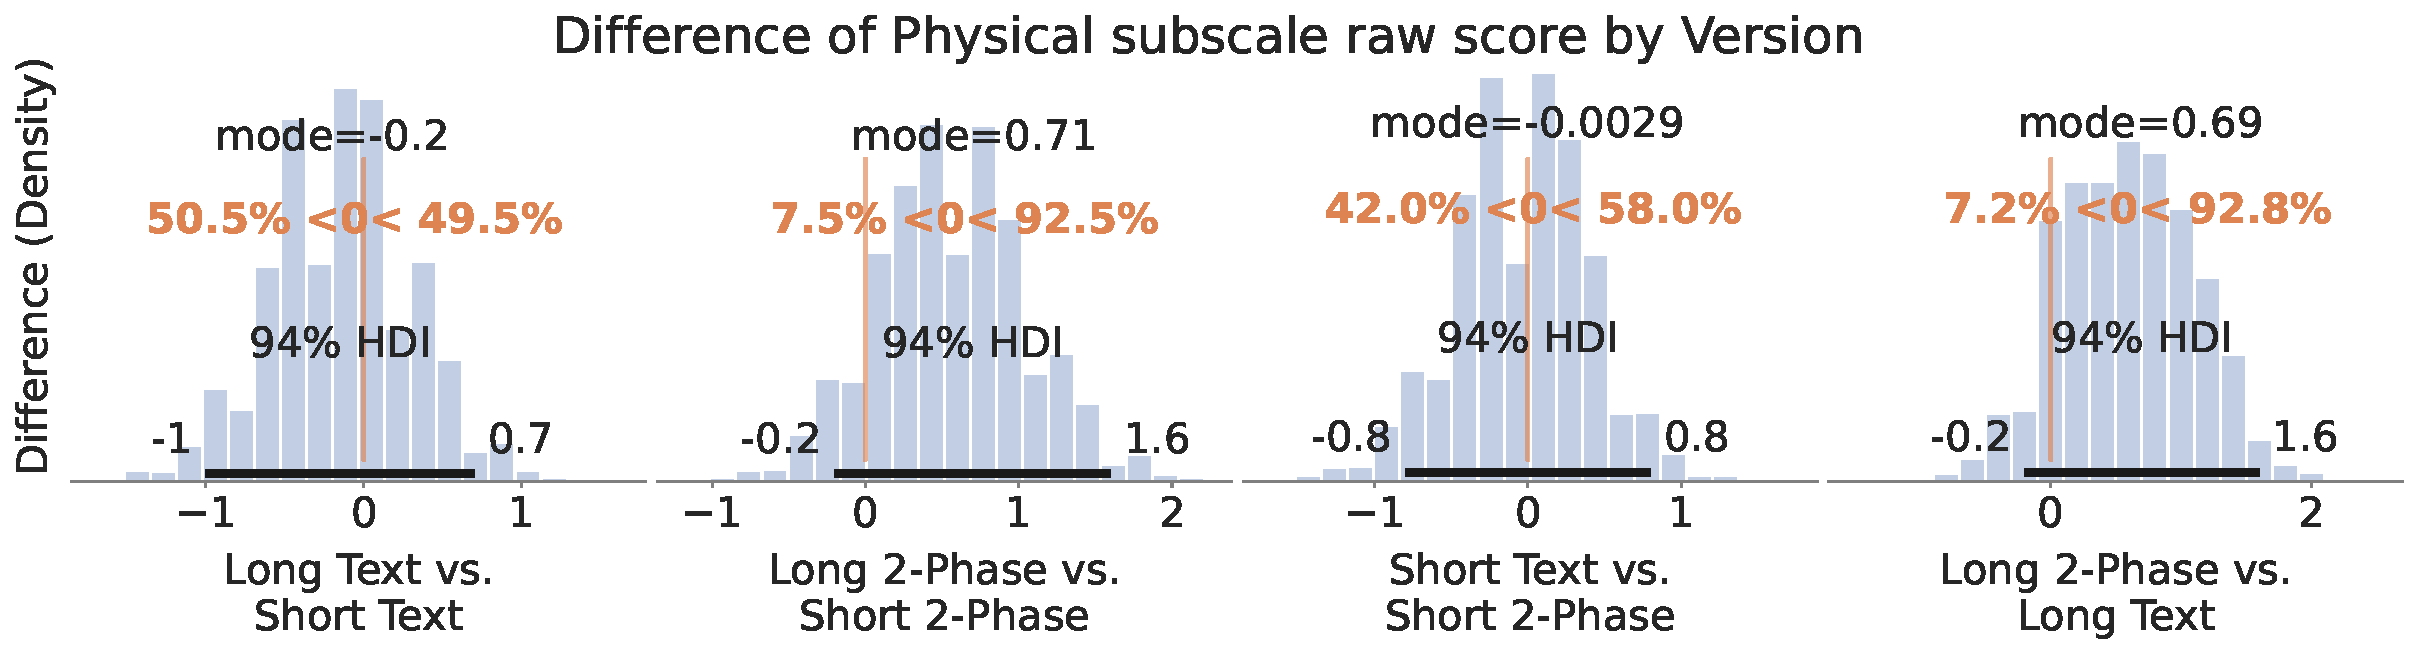
\includegraphics[width=0.75\textwidth]{content/image/cog/Physical_cog_diff_single_row.pdf}
    \caption{Differences in the physical subscale scores by version.~\textbf{Main Takeaway:} Participants in the long two-phase condition show trends to increase physical demand compared to short two-phase and long text despite the long text participants traversing higher edit distances.}
    \Description{A grouped panel of four histograms titled "Difference of Physical subscale raw score by Version," displaying posterior distributions of differences between various experimental conditions. Each plot shows a histogram of density (y-axis) versus difference (x-axis), with key summary statistics. Each histogram includes credible intervals, density curves, and a vertical line at zero for reference. Summary values are highlighted in orange and positioned at the top of each plot.}
    \label{fig:bayesian_physical_subscale}
\end{figure*}

\begin{figure*}[h!]
    \centering
    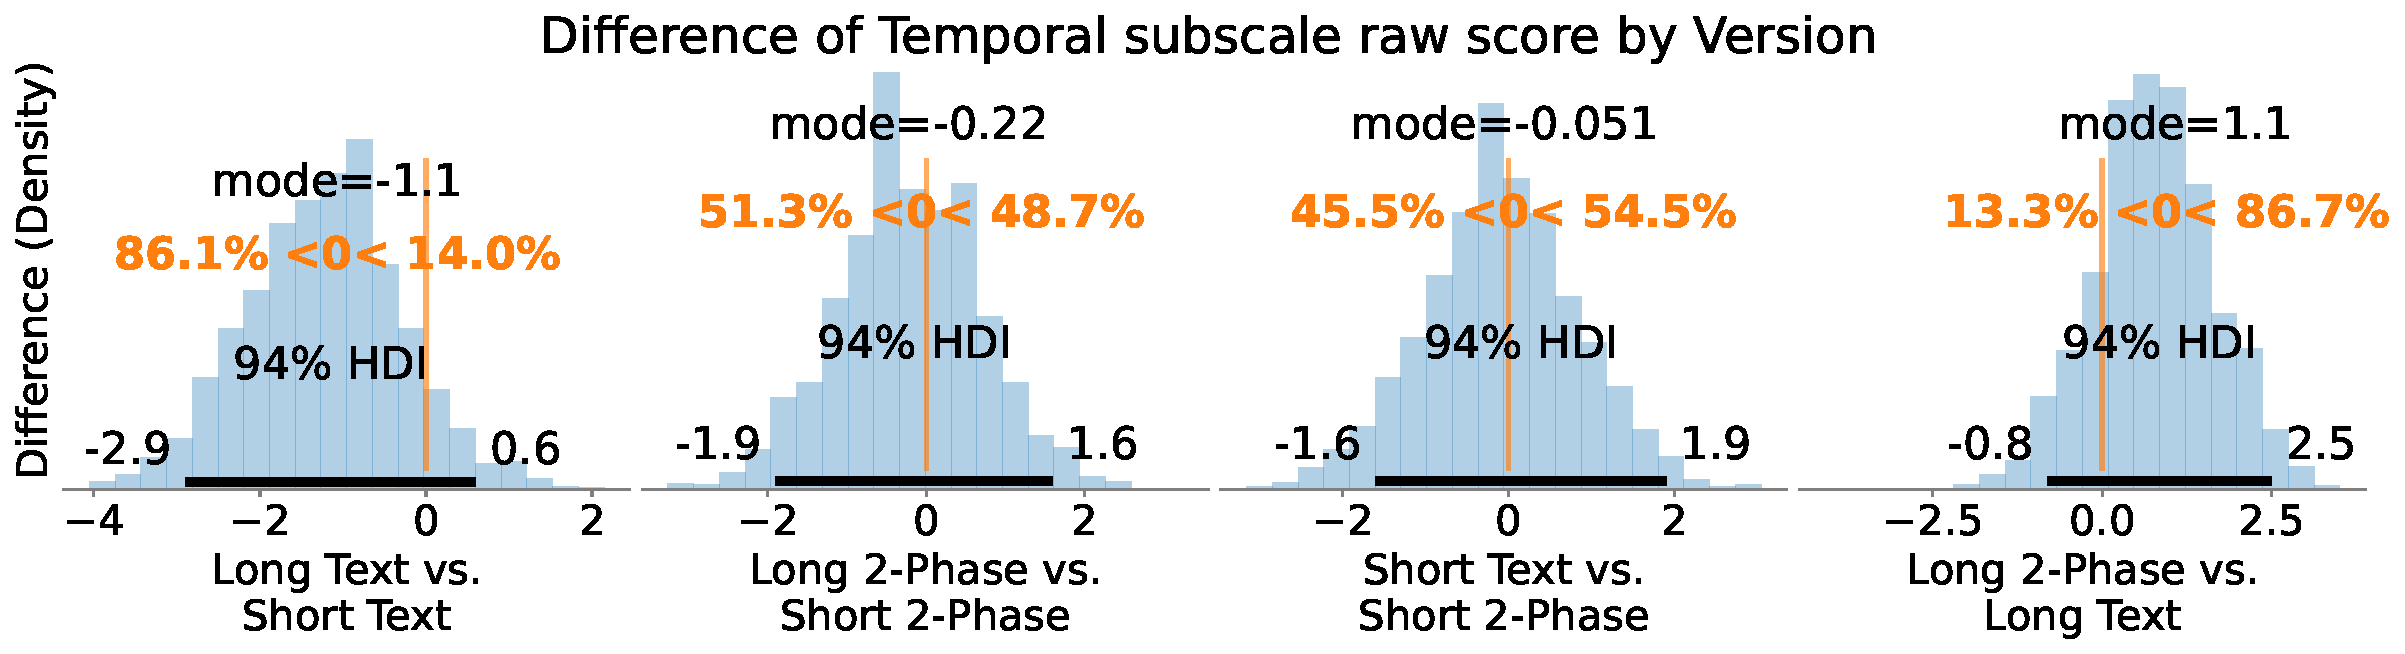
\includegraphics[width=0.75\textwidth]{content/image/cog/Temporal_cog_diff_single_row.pdf}
    \caption{Differences in the temporal subscale scores by version.~\textbf{Main Takeaway:} Participants in the long text condition show a trend that it reduces temporal demand compared to the short text condition and the long two-phase condition.}
    \Description{A grouped panel of four histograms titled "Difference of Temporal subscale raw score by Version," displaying posterior distributions of differences between various experimental conditions. Each plot shows a histogram of density (y-axis) versus difference (x-axis), with key summary statistics. Each histogram includes credible intervals, density curves, and a vertical line at zero for reference. Summary values are highlighted in orange and positioned at the top of each plot.}
    \label{fig:bayesian_temporal_subscale}
\end{figure*}

\begin{figure*}[h!]
    \centering
    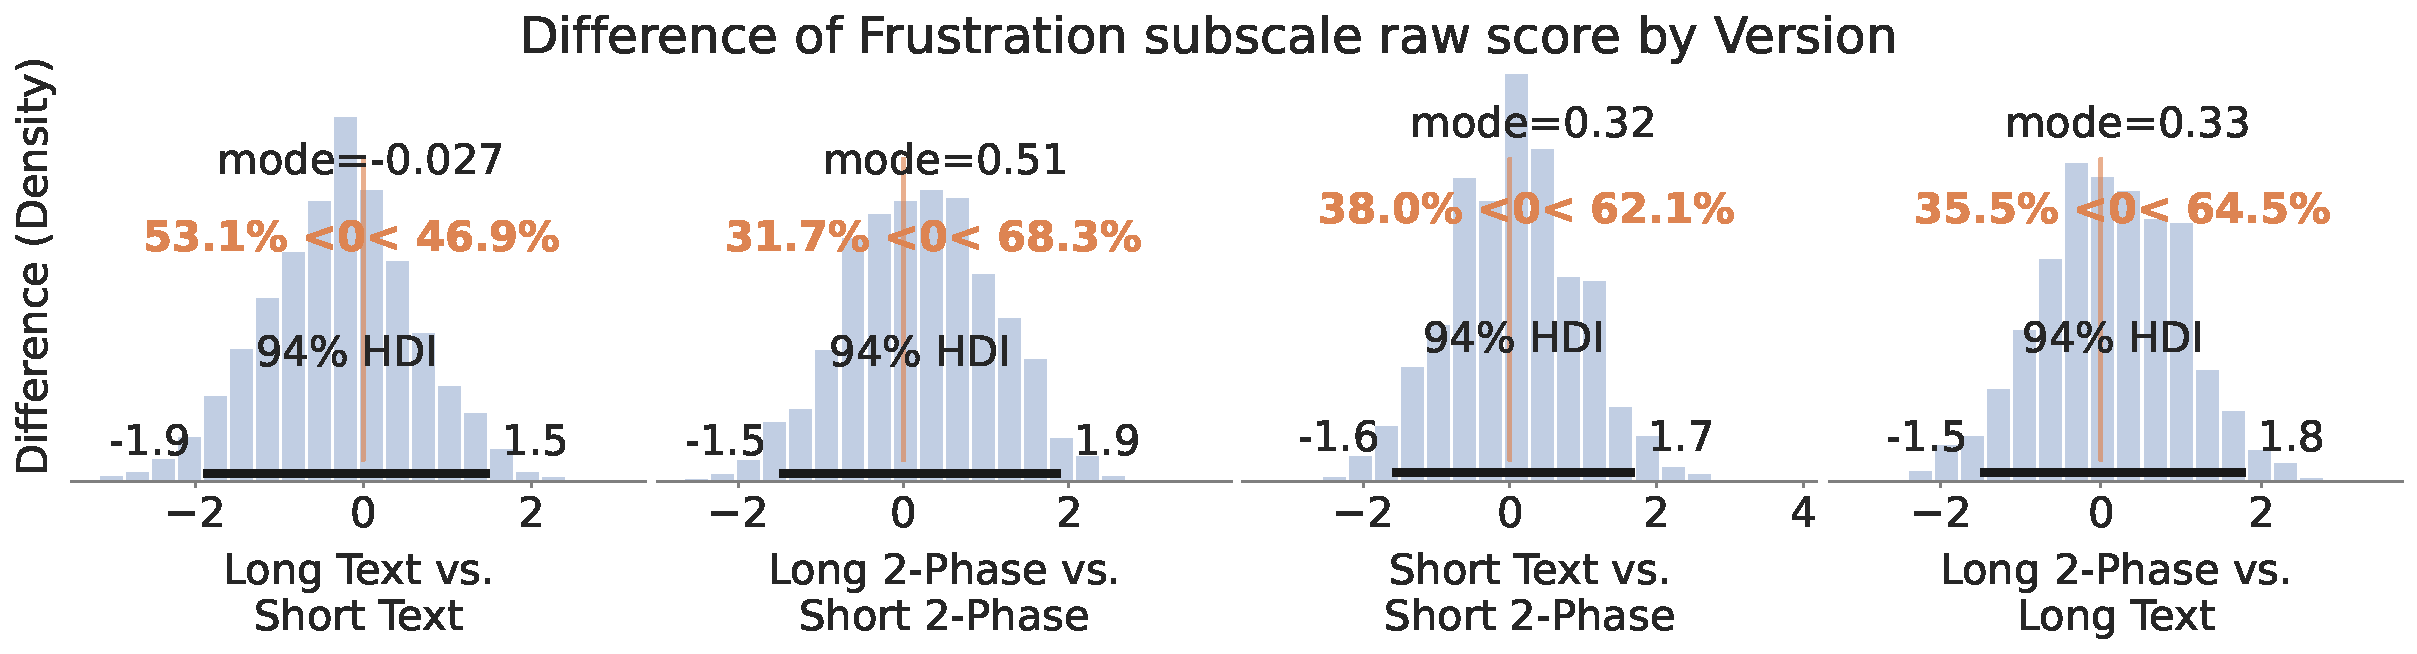
\includegraphics[width=0.75\textwidth]{content/image/cog/Frustration_cog_diff_single_row.pdf}
    \caption{Differences in the frustration subscale scores by version.~\textbf{Main Takeaway:} The model does not see a significant difference in the frustration subscale between experiment groups other than a trend for participants in the long two-phase condition to have higher frustration than the short two-phase participants.}
    \Description{A grouped panel of four histograms titled "Difference of Frustration subscale raw score by Version," displaying posterior distributions of differences between various experimental conditions. Each plot shows a histogram of density (y-axis) versus difference (x-axis), along with key summary statistics. The plots highlight the density and credible intervals for the differences, with key values marked in orange (percentages) and labeled at the top of each distribution. The vertical line at zero serves as a reference point.}
    \label{fig:bayesian_frustration_subscale}
\end{figure*}

% Section for Mental subscale
\subsubsection{Mental Subscale}
Figure~\ref{fig:bayesian_mental_subscale} shows pairwise Bayesian results from mental demand highlighted 70.4\% of posterior probability that participants in the long two-phase condition had a higher mental demand compared to the short two-phase condition. On the other hand, the short text condition had a 74.5\% posterior probability of having a higher mental demand compared to the short two-phase condition. This is additional evidence that prompted us to believe that the participants in the short two-phase participants benefited from the organization phase. The sheer number of added options in the long two-phase condition may have added additional demand to participants, leading to higher mental demand.

% Section for Physical subscale
\subsubsection{Physical Subscale}
Figure~\ref{fig:bayesian_physical_subscale} shows the pairwise comparison of the physical subscale. Notable results show that there is a 86.1\% posterior probability that the long text condition had a lesser physical demand compared to the short text condition. This is counter intuitive as the long text participants actually traversed much higher edit distances. We are not clear what prompted their self reported value and requires future research. 

% Section for Temporal subscale
\subsubsection{Temporal Subscale}
\label{sec:temporal_subscale_bayesian}
Figure~\ref{fig:bayesian_temporal_subscale} shows the pairwise comparison of the temporal subscale. The results show that the long two-phase condition once again had a 74.6\% posterior probability of having a lower temporal demand compared to the short text condition. Conversely, participants in the long two-phase condition had a 71.1\% posterior probability of having a higher temporal demand compared to the short two-phase condition, reflecting the longer time they took to complete the survey questions. We believe that the lower temporal demand in the long two-phase condition is potential indicator of the participants' satisficing behavior.

% Section for Performance subscale
\subsubsection{Performance Subscale}
We omit the pairwise comparison of the performance subscale due to the mixed signals. We focused on the qualitative results analyzed in the main text.

% Section for Effort subscale
\subsubsection{Effort Subscale}
We omit the pairwise comparison of the effort subscale due to its similarity to the mental demand subscale. 

% Section for Frustration subscale
\subsubsection{Frustration Subscale}
Figure~\ref{fig:bayesian_frustration_subscale} shows the pairwise comparison of the frustration subscale. The results show that the long two-phase condition had a 68.3\% posterior probability of having a higher frustration compared to the short two-phase condition, likely due to the added number of options to assess. 

